%%%%%%%%%%%%%%%%%%%%%%%%%%%%%%%%%%%%%%%%%
% Short Sectioned Assignment
% LaTeX Template
% Version 1.0 (5/5/12)
%
% This template has been downloaded from:
% http://www.LaTeXTemplates.com
%
% Original author:
% Frits Wenneker (http://www.howtotex.com)
%
% License:
% CC BY-NC-SA 3.0 (http://creativecommons.org/licenses/by-nc-sa/3.0/)
%
%%%%%%%%%%%%%%%%%%%%%%%%%%%%%%%%%%%%%%%%%

%----------------------------------------------------------------------------------------
%	PACKAGES AND OTHER DOCUMENT CONFIGURATIONS
%----------------------------------------------------------------------------------------

\documentclass[paper=a4, fontsize=11pt]{scrartcl} % A4 paper and 11pt font size

\usepackage[T1]{fontenc} % Use 8-bit encoding that has 256 glyphs
%\usepackage{fourier} % Use the Adobe Utopia font for the document - comment this line to return to the LaTeX default
\usepackage[english]{babel} % English language/hyphenation
\usepackage{amsmath,amsfonts,amsthm} % Math packages

\usepackage{lipsum} % Used for inserting dummy 'Lorem ipsum' text into the template

\usepackage{sectsty} % Allows customizing section commands
\allsectionsfont{ \normalfont\scshape} % Make all sections centered, the default font and small caps

\usepackage{graphicx}
\usepackage{booktabs}
\usepackage[framed,numbered,autolinebreaks,useliterate]{mcode}

\usepackage{fancyhdr} % Custom headers and footers
\pagestyle{fancyplain} % Makes all pages in the document conform to the custom headers and footers
\fancyhead{} % No page header - if you want one, create it in the same way as the footers below
\fancyfoot[L]{} % Empty left footer
\fancyfoot[C]{} % Empty center footer
\fancyfoot[R]{\thepage} % Page numbering for right footer
\renewcommand{\headrulewidth}{0pt} % Remove header underlines
\renewcommand{\footrulewidth}{0pt} % Remove footer underlines
\setlength{\headheight}{13.6pt} % Customize the height of the header

\numberwithin{equation}{section} % Number equations within sections (i.e. 1.1, 1.2, 2.1, 2.2 instead of 1, 2, 3, 4)
\numberwithin{figure}{section} % Number figures within sections (i.e. 1.1, 1.2, 2.1, 2.2 instead of 1, 2, 3, 4)
\numberwithin{table}{section} % Number tables within sections (i.e. 1.1, 1.2, 2.1, 2.2 instead of 1, 2, 3, 4)

\setlength\parindent{0pt} % Removes all indentation from paragraphs - comment this line for an assignment with lots of text

%----------------------------------------------------------------------------------------
%	TITLE SECTION
%----------------------------------------------------------------------------------------

\newcommand{\horrule}[1]{\rule{\linewidth}{#1}} % Create horizontal rule command with 1 argument of height

\title{	
\normalfont \normalsize 
\textsc{APSC 1001, George Washington University} \\ [25pt] % Your university, school and/or department name(s)
\horrule{0.5pt} \\[0.4cm] % Thin top horizontal rule
\huge APSC 1001 MATLAB Curve Fitting Tools \\ % The assignment title
\horrule{2pt} \\[0.5cm] % Thick bottom horizontal rule
}

\author{\normalsize Randy Schur } % Your name

%\normalsize Week 1 Handout
\date{\normalsize \today } % Today's date or a custom date


\begin{document}

\maketitle % Print the title

\section{Sampling Data}
An valuable part of your toolbox of engineering skills is testing, data collection, and analysis.
Much of what scientists and engineers study was originally discovered by experimentation and the analysis of experimental data.
The ability to decipher some meaning from the data you collect is something you will rely on throughout your engineering career. 

\subsection{Signal Analysis}
Many textbooks have been written on the analysis of different types of signals, and we won't go into great detail in this class.
Some common examples of applications that demand signal analysis are circuit design and radio frequency (RF) work in electrical engineering, image processing in computer science, wind or water tunnel experiments in mechanical or aerospace engineering, and earthquake movement in civil engineering. 

Often, the signals we see are repeating. 
We call this \textit{periodic}, meaning that the signal is repetitive and has a measurable period, or length of time between cycles.
The simplest example of a periodic signal is a sine wave. 
In fact, any periodic signal may be replicated using only sine (or cosine) waves of different frequencies!
This is a surprising and extremely important result in many fields of mathematics and engineering. 
Breaking a signal up into its component frequencies is called a Fourier Transform, named after Joseph Fourier who (sort of) discovered that periodic, or \textit{sinusoidal}, functions can be approximated by sine waves.
It is something that you will likely discuss in several classes during your studies.  

\subsection{Statistical Approximations}
Not all data that we collect is from a periodic signal. Sometimes we have a single process, and we test it multiple times while changing one or more variables. 
An example of a data collection task like this might be testing for when a particular component fail. 
You might vary the loading on that component, and run the test multiple times. 
Once you have collected data from multiple runs of the experiment, you might try to find the how the failure of the component depends on the loading. 
You are looking for a \textit{function} for failure in terms of loading. 
Because we can't perfectly control any experiment, there will be some element of randomness to the data you collect. 
However, using some statistical tools, it it often possible to find a relationship between the two (or more) variables that you observing.
This process is called \textit{curve fitting}.

\section{Curve Fitting in MATLAB}
MATLAB provides several built in functions that can help with curve fitting.
We are going to use a tool with a nice GUI called cftool.
See the example below to learn how to use this tool.

One way we can test the tool is to make up a function, inject some randomness in order to model 'experimental' data, and then see if we can find the original function.

Type the following into MATLAB.
\begin{verbatim}
>> x = linspace(0,100,101); %create initial data
>> y_actual = 2.5*x + 17; %function of x
>> rnums = 15*randn(1, 101); %random numbers with a zero mean (no bias)
>> y_test = y_actual + rnums; %create 'test' data.
\end{verbatim}

Now we'll use the curve fitting toolbox to see if we can get the correct function from our test data.
\begin{verbatim}
>> cftool(x, y_test)
\end{verbatim}

This brings up the curve fitting GUI. The screen shot below has several important values highlighted, which MATLAB often fills out automatically. 
The first is the type of curve that we are looking for, which in this case is a first degree polynomial.
The next important part is the selection of data that we are using - it is good to confirm the correct data is being used for the x and y axis.
Below the variables is the results section, where you can find the function that MATLAB has generated, and the coefficients to go along with that function.
Also located in that box is a section titled Goodness of Fit. 
The value we are interested in is the R-square value, which can act as an estimate of how well the generated curve fits the data set.
A value closer to 1 means a better fit.
Finally, there is a plot of the data and the of the curve.
Notice that the data is plotted as discrete points, while the function is plotted as a continuous line. 
This is conventional; test data should always be plotted discretely and functions should be plotted as continuous.

\begin{figure}[h!]
\centering
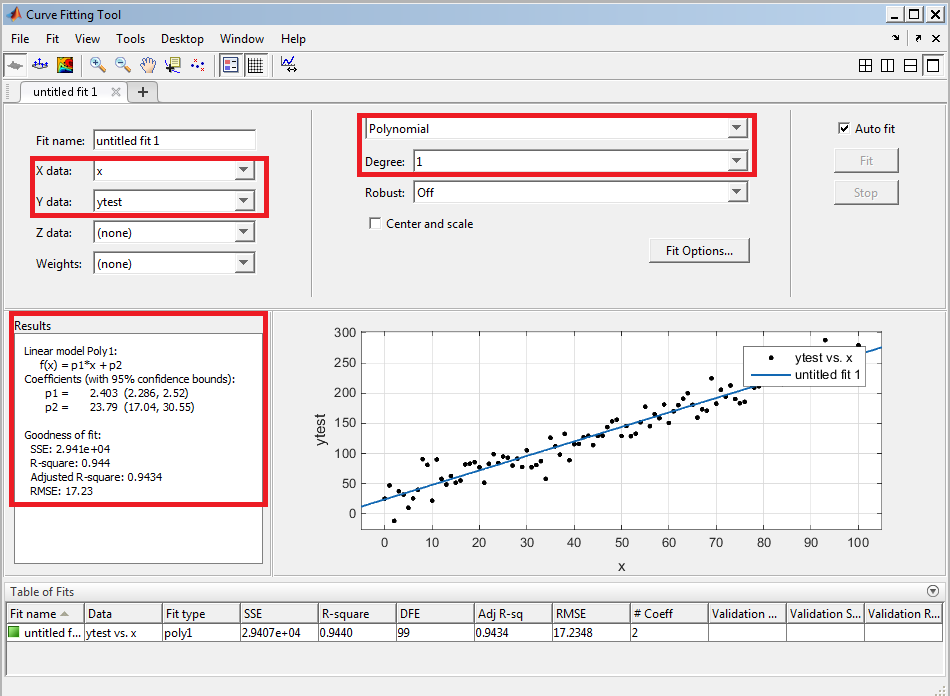
\includegraphics[scale=.65]{cftool_screenshot}
\caption{MATLAB's curve fitting toolbox GUI.}
\end{figure}

There are several ways to save the generated curve so that we can use it in a script or the command window. 
Here, we are going to save the coefficients as variables, and then plot the curve again on our own.
So, in this case we would type into the command window: 
\begin{verbatim}
>> p1 = 2.403;
>> p2 = 23.79;
\end{verbatim}
For a first degree polynomial, this is all the information we will need!

Now, if we want to plot the generated curve there are two options. 
The first is to create an array containing a y value for each x value. 
\begin{verbatim}
>> y_curve_fit = p1*x + p2;
\end{verbatim}
Then, we can plot x vs. y\_curve\_fit on the same plot as x vs. y\_test, and recreate the plot we saw in the curve fitting tool. 
Try this, and create a title, axis labels, and legend. 
Does your plot match the one in the tool? Why might it be useful to create your own plot rather than use the one in the toolbox?

\subsection{Writing a function}
There is another option for generating the values in y\_curve\_fit. 
MATLAB has many built in functions, but we can also write our own.
Type the following line into the command window:
\begin{verbatim}
>> f = @(s) p1*s + p2;
\end{verbatim}
We have just written our first MATLAB function!
Now, we can do the following: 
\begin{verbatim}
>> y_generated = f(x);
\end{verbatim}
Our function, f, takes an argument of a vector and returns a vector representing our fitted curve.
In addition to using x, we could create any array we want and run it through our function.
The result would be a segment of the line generated by the curve fitting toolbox. 
Try creating a new x vector that has values from 0 to 1000, and use this function to generate y values. 
Then, plot the result on the same graph as the original data set. 
Why might this be useful?

\end{document}
